\documentclass[a4paper]{article}
\usepackage[utf8]{inputenc}
\usepackage[english, portuguese]{babel}
\usepackage{amsmath}
\usepackage{geometry}
\usepackage{graphicx}
\usepackage{hyperref}
\usepackage{xcolor}

\geometry{
    a4paper,            % Page Size
    left    =20mm,      % Left   Margin
    right   =20mm,      % Right  Margin
    bottom  =20mm,      % Bottom Margin
    top     =20mm,      % Top    Margin
    marginparwidth=50mm %
}



\author{Guilherme Nunes Trofino - 217276}
\title{MC521B - Relatório 20260227}

\begin{document}

\maketitle
\section{\href{https://atcoder.jp/contests/abc258/tasks/abc258_c}{C-P03 from AtCoder abc258C}}
\paragraph{Descrição} Neste problema são providas as variáveis \texttt{N}, \texttt{Q} e \texttt{S} representando respectivamente: a quantidade de caracteres da palavra \texttt{S}, a quantidade de operações a serem realizadas e uma palavra composta de caracteres minúsculos em inglês. Há 2 duas operações possíveis:

\begin{itemize}
    \item \texttt{1 x}: repetindo \texttt{x} vezes o processo de remover o último caracter de \texttt{S} e adicioná-lo ao início do mesmo.
    \item \texttt{2 x}: imprimir o \texttt{x}-ésimo caracter de \texttt{S}
\end{itemize}


\subsection{Solução}

\paragraph{Inicialização} Após recuperar as entradas \texttt{N}, \texttt{Q} e \texttt{S} inicializa-se \texttt{reference} em zero como variável auxiliar para registrar as operações de remoção e adição dos carateres de \texttt{S}.

\paragraph{Execuções} Na sequência o algoritmo entrará em repetição através de um \texttt{loop} pela quantidade \texttt{Q} de operações explicitadas tratando uma operação por vez de acordo com as opções anteriormente descritas:

\begin{itemize}
    \item caso seja uma operação \texttt{1 x}: a variável \texttt{reference} será incrementada em \texttt{x}.
    \item caso seja uma operação \texttt{2 x}: será imprimido o caracter na posição correspondente a equação abaixo:
    \begin{equation}
        \texttt{S}
        [
            \underbrace{
                \underbrace{
                    (
                        \underbrace{
                            \texttt{int(x) - reference}
                        }_{\text{translação}}
                    ) \texttt{ \% len(S)}
                }_{\text{circular}}
                    - 1
            }_{\text{correção de indice}}
        ]
    \end{equation}
\end{itemize}
Quando uma operação \texttt{1 x} é realizada, a palavra será essencialmente "transladada" circularmente. Desta forma, não há necessidade de modificar \texttt{S}, trata-se apenas de acessar o indice correspondente corrigido como mostram os exemplos abaixo:
\begin{itemize}
    \item \texttt{reference = 0}: \textcolor{black}{\texttt{ornitorinco}}
    \item \texttt{reference = 1}: \textcolor{gray}{\texttt{o}}\textcolor{black}{\texttt{ornitorinc}}
    \item \texttt{reference = 2}: \textcolor{gray}{\texttt{co}}\textcolor{black}{\texttt{ornitorin}}
\end{itemize}

\paragraph{Translação} Quando \texttt{reference = 2}, a operação \texttt{2 1} retornará o caracter de indice 1 de \textcolor{gray}{\texttt{c}}\textcolor{red}{\texttt{o}}\textcolor{black}{\texttt{ornitorin}} representado em vermelho que seria equivalente ao caracter de indice -1 de \textcolor{black}{\texttt{ornitorinc}}\textcolor{red}{\texttt{o}} representado em vermelho quando \texttt{reference = 0}, justificando a seção de translação da equação acima.

\paragraph{Circular} Como as sucessivas operações podem acumular valores superiores a quantidade de caracteres de \texttt{S} se faz necessário utilizar apenas o resto da divisão inteira, justificando a seção de circular da equação acima.

\paragraph{Correção de Indice} Visto que a linguagem Python utilizada inicia sua referência em zero se faz necessário corrigir os indices, justificando a seção de correção de indice da equação.



\newpage
\section{\href{https://atcoder.jp/contests/abc267/tasks/abc267_b}{E-P05 from AtCoder abc267B}}

\paragraph{Descrição} Neste problema o estado de 10 pinos de boliche são fornecidos através da variável \texttt{S}, uma palavra de tamanho 10 caracteres em que cada caracter representa o estado do n-ésimo pino:
\begin{itemize}
    \item \texttt{0}: n-ésimo pino está \textbf{derrubado}.
    \item \texttt{1}: n-ésimo pino está \textbf{levantado}.
\end{itemize}
Considera-se que esses pinos podem ser agrupados por colunas como demonstrado na representação abaixo:
\begin{figure}[h]
    \centering
    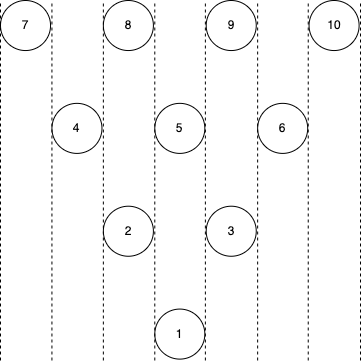
\includegraphics[height = 4cm]{pictures/atcoder_abc267b.png}
    \caption{Distribuição de Colunas dos Pinos de Boliche}
\end{figure}

\noindent Finalmente, considera-se que há uma separação nas colunas quando as seguintes condições são satisfeitas simultaneamente:
\begin{enumerate}
    \item pino 1 está derrubado
    \item há duas colunas diferentes que atendem simultaneamente as seguintes condições:
    \begin{itemize}
        \item cada coluna possui pelo menos 1 pino levantado
        \item existe uma coluna entre essas colunas em que todos os pinos estão derrubados
    \end{itemize}
\end{enumerate}

\subsection{Solução}

\paragraph{Inicialização} Após recuperar a configuração dos pinos pela leitura da variável \texttt{S}, inicia-se com a análise do estado do pino 1. Caso a pino 1 não esteja derrubado, a função retornará imediatamente que a configuração não possui uma separação evitando assim cálculos desnecessários.\\

\noindent Na sequência, converte-se os estados dos pinos em estados de colunas de forma que cada coluna seja representada pela soma dos estados dos pinos que a compõem. Dessa forma, considera-se a seguinte nomenclatura:
\begin{itemize}
    \item uma coluna \textbf{levantada}: possui ao menos um pino levantado
    \item uma coluna \textbf{derrubada}: não possui pinos levantados
\end{itemize}

\paragraph{Separação} Percorre-se as colunas entre a segunda e a penúltima inclusive buscando se há uma posição em que a coluna em questão está derrubada, há pelo menos uma coluna a esquerda levantada e há pelo menos uma coluna uma coluna a direita levantada, o que configura uma separação.\\

\noindent Caso uma separação seja encontrada, as interações são interrompidas e o resultado é apresentado. Se nenhuma separação for encontrada, o algoritmo retornará que não há separação.

\end{document}
